\chapter{Actuators modelling and control}\label{chap: modeling}
A widely used actuation system is reaction wheels which are spinning wheels and can exchange momentum with the spacecraft by increasing or decreasing the wheels speed. The rate of rotation can be adjusted by an electric motor and the magnitude of the wheels output torque is limited by the motors shaft torque. This chapter will provide characteristics of the chosen reaction wheels and BLDC motors along with the electrical and mechanical modelling of the motors for simulation purposes. 
%
\section{Reaction wheels}
%
%Since the focus of the current thesis is not on the design of reaction wheels, only few constraints are  taken into account for the selection of the wheels, such as the weight and the inertia. In order to minimize the total weight of the satellite, the weight of each wheel, is not overcome the %weight of each motor. 

The satellite should be capable of tracking an Earth station in order to be able to downlink data effectively. Tracking a ship requires similar control capability, since the velocity of the wheel is practically zero compared to the velocity of the satellite. Directing the antennas to the nadir continuously only requires keeping a satellite angular velocity equal to the orbit's angular velocity.
Tracking the Earth station requires torque from the actuators, the torque demand can be calculated based on the angular acceleration demand for Earth station tracking.


 The reaction wheels are chosen to give higher inertia from the motor shaft, and can provide medium manoeuvrability in terms of time required to turn the satellite $90^o$ \cite{SIDI}. The wheel inertia is \cite{flywheel_design_thesis} $J_{wheel} = 2.456 [gcm^2]$ and the weight is $m_{wheel} = 4.201 [g] $ compared to the motor weight $m_{motor} =8 [g] $ and the motor shaft inertia $J_{motor} = 0.0249 [gcm^2]$. The characteristics of the selected motor can be found in appendix \ref{chap: B}. The maximal speed of the motor is $\omega_{max}= 20000[rpm]$ and thus the maximum angular momentum that the system wheel-motor can provide can be found as    
%
%\nomenclature[S]{\textbf{$J_{wheel}$}}{Reaction wheel inertia}
%\nomenclature[S]{\textbf{$J_{motor}$}}{Motor inertia}
%\nomenclature[S]{\textbf{$m_{motor}$}}{Weight of the motor}
%\nomenclature[S]{\textbf{$m_{wheel}$}}{Weight of the reaction wheel}
\begin{flalign*}
	h_{max} = {J_{wheel}} {\omega_{max}} 
\end{flalign*}
%\nomenclature[S]{\textbf{$h_{max}$}}{Maximum angular momentum of the wheel-motor system}
%0.000114450   5.1438e-04
which is found to be $5.1438*10^{-4} [Kgm^2/s]$ for each wheel.	
%
%
For 3 axis stabilization, 3 wheels each orthogonal to the principal axis, are efficient but lack of robustness is present if one actuator fails. Redundancy is desired, requiring four wheels in tilted positions. The configuration of the wheels is chosen to be in tetrahedron shape giving rise to more reliable and robust system. The tetrahedron configuration will be discussed in chapter \ref{ref:reactConfig}.  
\subsection{BLDC motor model}
\label{sec:motors}

In order to make the system more reliable, brush-less DC motors are chosen as actuators. BLDC motors are lighter compared to brushed with the same power output and do not causing sparking thus can be used in operations that demand long life and reliability.
%
%\nomenclature[A]{\textbf{BLDC}}{Brushless Direct Current }
Each motor consists of an electrical part and a mechanical part. The electrical part of the motor can be modeled using Kirchhoff's Voltage Law as
%
\begin{flalign}
 V_{a} -V_{R}-V_{L} -V_{e} = 0
\label{Kirchhoff1}
\end{flalign}
%
%\nomenclature[S]{\textbf{$V_{a}$}}{Voltage source }
%\nomenclature[S]{\textbf{$V_{R}$}}{Voltage drop across the resistance }
%\nomenclature[S]{\textbf{$V_{L}$}}{Voltage drop across the inductance }
where $V_{a}$ is the voltage source, $V_{R}$ is the voltage drop across the resistance, $V_{L}$ is the voltage drop across the inductance and $V_{e}$ is the back emf. \Eqref{Kirchhoff1} can be re written as 
%
%\nomenclature[S]{\textbf{$V_{e}$}}{Back electromotive force- emf }
\begin{flalign}
	V_{a}= R_{a}i + L_{a}\dfrac{di}{dt}+ k_{e}\omega
	\label{Kirchhoff244}
\end{flalign}
%
%\nomenclature[S]{\textbf{$R_{a}$}}{Armature resistance}
%\nomenclature[S]{\textbf{$L_{a}$}}{Armature inductance}
%\nomenclature[S]{\textbf{$k_{e}$}}{Back emf coefficient}
 where $R_{a}$ [Ohm] is the armature resistance, $L_{a}$ [H] is the armature inductance and $k_{e}$ is the back emf coefficient as it can be seen in the \figref{fig:electromech} .   
%

\begin{table}[H]
	\begin{minipage}[b]{0.49\linewidth}
		\centering
		\begin{figure}[H]
			\centering
			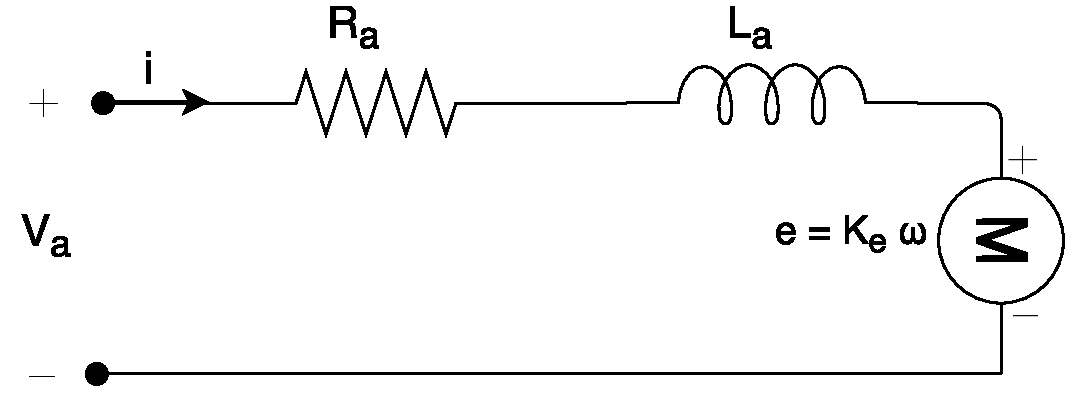
\includegraphics[width=1\linewidth]{figures/BLDC_el.pdf}
			%\caption{ Electrical and mechanical part of the motor }
		%	\label{fig:electromech}
		\end{figure}
	\end{minipage}\hfill
	\begin{minipage}[b]{0.49\linewidth}
		\centering
		\begin{figure}[H]
			\centering
			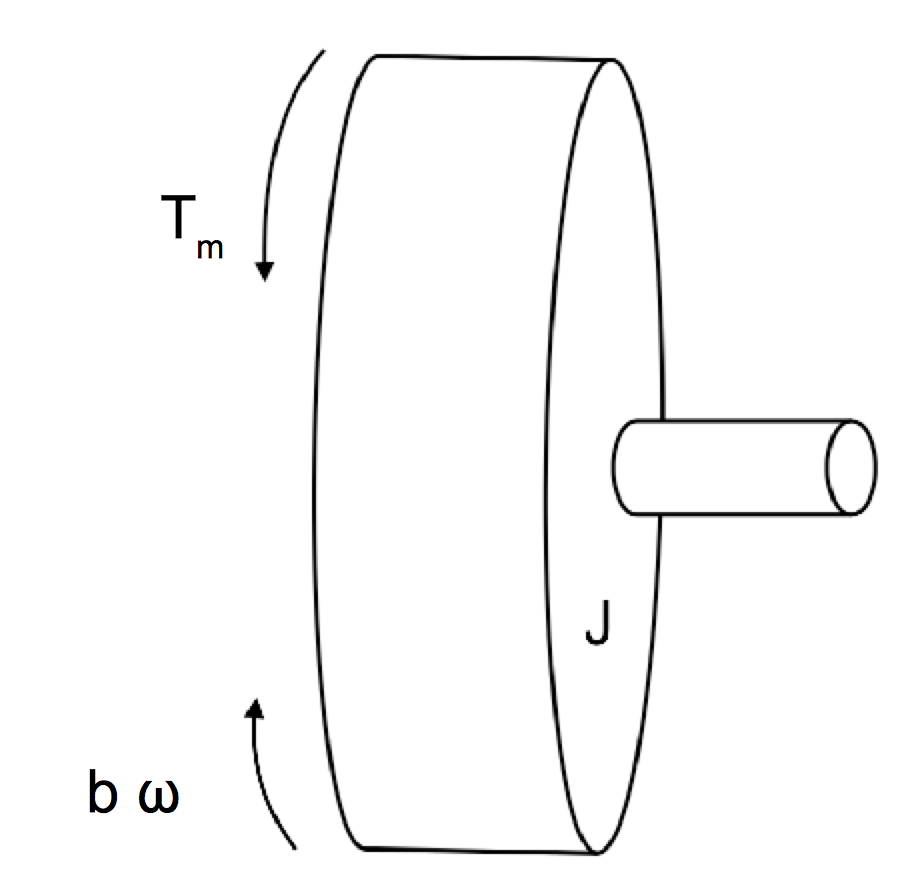
\includegraphics[width=0.55\linewidth]{figures/flywheel_1}
			%\caption{Mechanical part of the motor}
			%\label{fig:distancecontrol4}
		\end{figure}
	\end{minipage}
	\caption{ Electrical and mechanical part of the motor }
	\label{fig:electromech}
\end{table}

%
The mechanical part of the motor can be modelled as 
%
\begin{flalign}
 k_{t}i  =J\dfrac{d\omega}{dt} + b\omega
	\label{mechpart66}
\end{flalign}
%
%\nomenclature[S]{\textbf{$k_{t}$}}{Motor torque coefficient}
%\nomenclature[S]{\textbf{$b$}}{Viscous friction coefficient}
where $J$ is the rotor moment of inertia, $k_{t}$ [Nm/A] is the motor torque coefficient and $b$ [Nm s/rad] is the viscous friction coefficient. %Assuming the current will not increase rapidly in order not to harm the equipment, and moreover the electrical time constant $\tau_{e}=\dfrac{L}{R}$ is much smaller than the mechanical time constant $\tau_{m}=\dfrac{J}{b}$, the effect of the inductance can be neglected and the
 \Eqref{mechpart66} can be solved for $i$ and  replaced in \eqref{Kirchhoff244}\cite{permanent_magnet}     
%
\begin{flalign}
	i  =\dfrac{J}{k_{t}}\dfrac{d\omega}{dt} + \dfrac{b}{k_{t}}\omega
	\label{mechpart2}
\end{flalign}
%
\begin{flalign}
 V_{a} = \dfrac{LJ}{k_{t}}\dfrac{d^{2}\omega}{dt^{2}}+\dfrac{RJ+Lb}{k_{t}}\dfrac{d\omega}{dt} +\dfrac{Rbk_{e}}{k_{t}}\omega 
	\label{mechpart333}
\end{flalign}
%
by laplace transformed \eqref{mechpart333}, the second order transfer function from $V_{a}$ to $ \omega $ can be written as 
%
\begin{flalign}
	\dfrac{\omega(s)}{V_{a}(s)}= \dfrac{k_{t}}{LJs^{2}+(RJ+Lb)s+(Rb+k_{e}k_{t})}
	\label{tf}
\end{flalign}
%= \dfrac{k_{t}}{LJs^{2}+(RJ+Lb)s+Rb+k_{e}k_{t}}
%\label{tf}
following \cite{permanent_magnet} the electrical time constant $\tau_{e}$ and mechanical time constant $\tau_{m}$ can be written respectively $\tau_{e} = \frac{LJ}{RJ+Lb}$ and $\tau_{m} = \frac{RJ+LB}{RB+k_{e}k_{t}}$, the values for the two time constants are found to be $\tau_{e} = 1.2709*10^{-10}$[s] and $\tau_{m} = 8.4102*10^{-4}$[s] thus since the $\tau_{e}$ is very small compared to $\tau_{m}$, the effect of inductance can be though negligible thus the transfer function from $V_{a}$ to $ \omega $ is reduced to a first order transfer function as 
%
\begin{flalign}
\dfrac{\omega(s)}{V_{a}(s)}= \dfrac{k_{t}}{R(Js+b)+k_{e}k_{t}}
\label{tf2}
\end{flalign}
%
the block diagram of the system can be seen in \figref{fig:blockdi} along with PI velocity controller which will be discussed in the next chapter. Four wheels, requiring four motors in tetrahedron configuration. The total moment of inertia of the motor-wheel system is the sum of individual moments $J = J_{wheel}+J_{motor}$. Since $J_{wheel}\gg J_{motor}$ the inertia of the motor can be neglected.
%
%\nomenclature[S]{\textbf{$\tau_{e}$}}{Electrical time constant}
%\nomenclature[S]{\textbf{$\tau_{m}$}}{Mechanical time constant}
\begin{figure}[H]
	\centering
	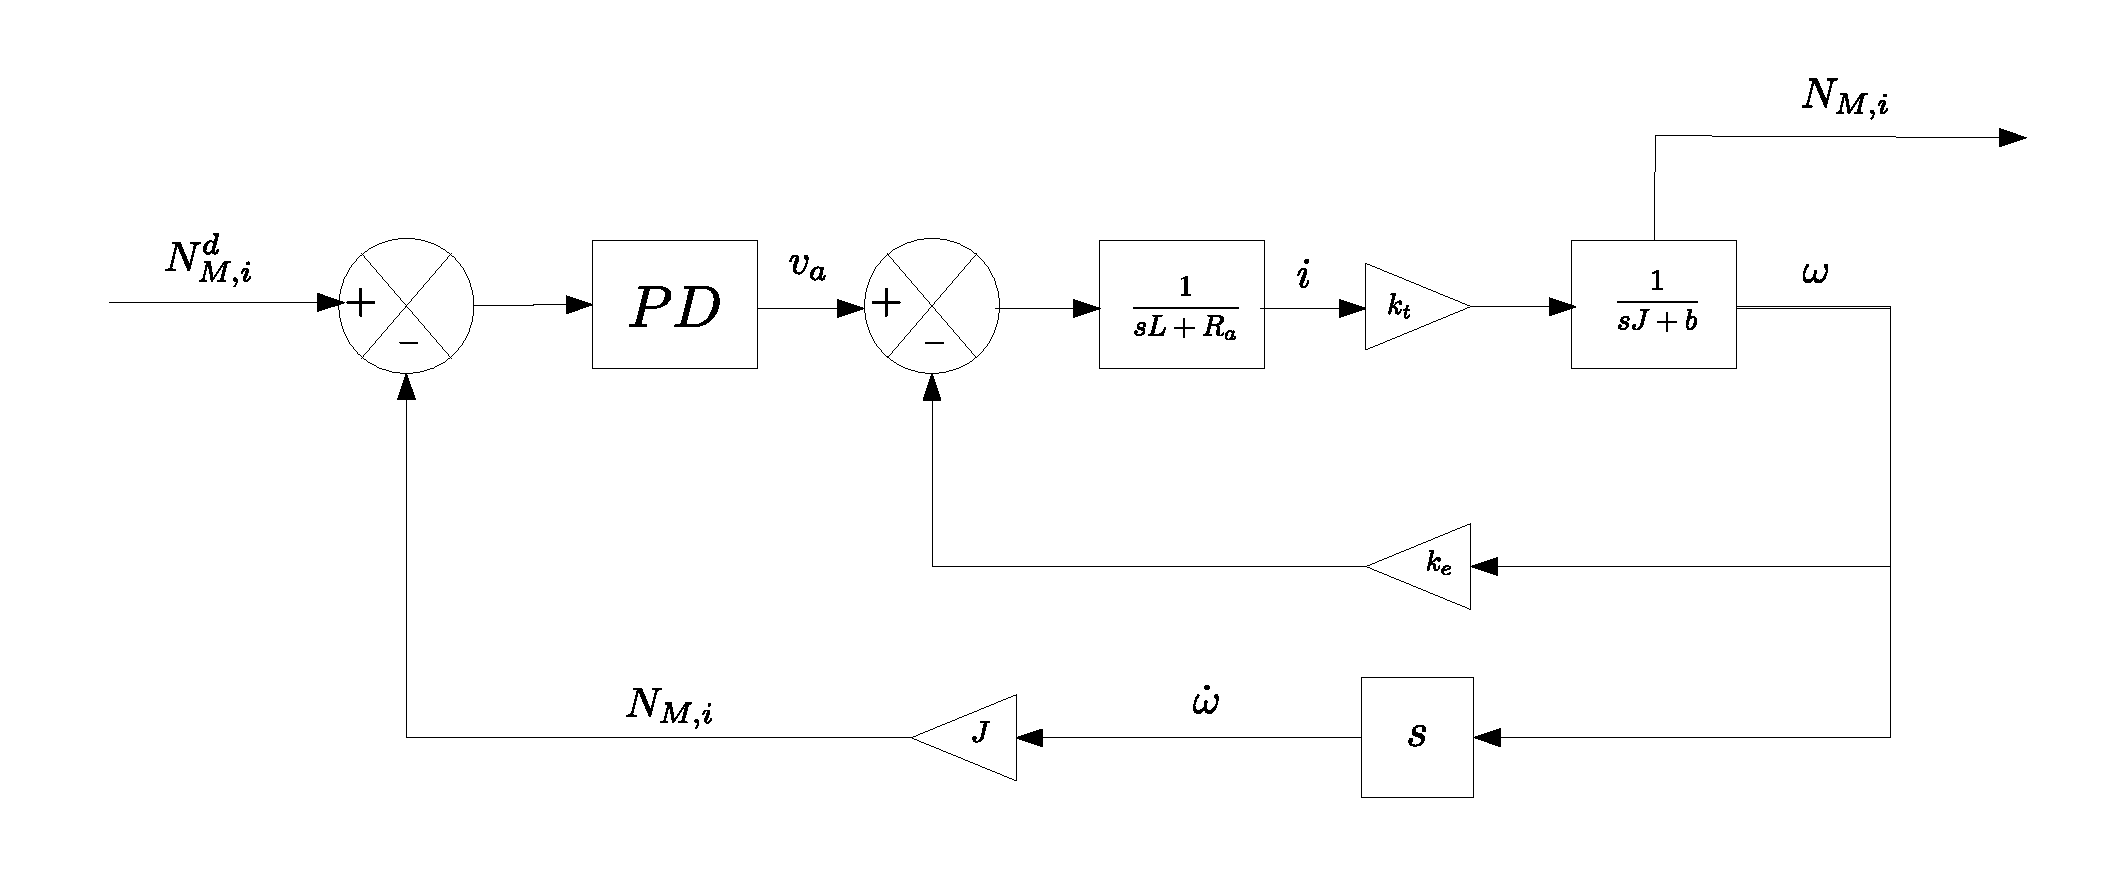
\includegraphics[width=0.9\linewidth]{figures/omegaControl}
	\caption{Angular velocity controlled DC motor}
	\label{fig:blockdi}
\end{figure}
%

% 
\chapter{Motor control}

\subsection*{ Angular velocity control}

In previous work, two controllers a linear and a non-linear(SMC), have been designed requiring a torque that has to be produced from the motors-wheel system. This torque demand is used to give the desired angular velocity reference for the wheels and thus the torque that will be fed back to the satellite as seen in the \cite{block diagram}. The output torque from the linear and non-linear controllers has three elements which has to be transformed in the tetrahedron configuration using the matrix \eqref{transmatrix}.  A \textit{PID} controller has been designed to control the angular velocity of the motor as seen in the \figref{fig:blockdi222}:
\begin{figure}[H]
	\centering
	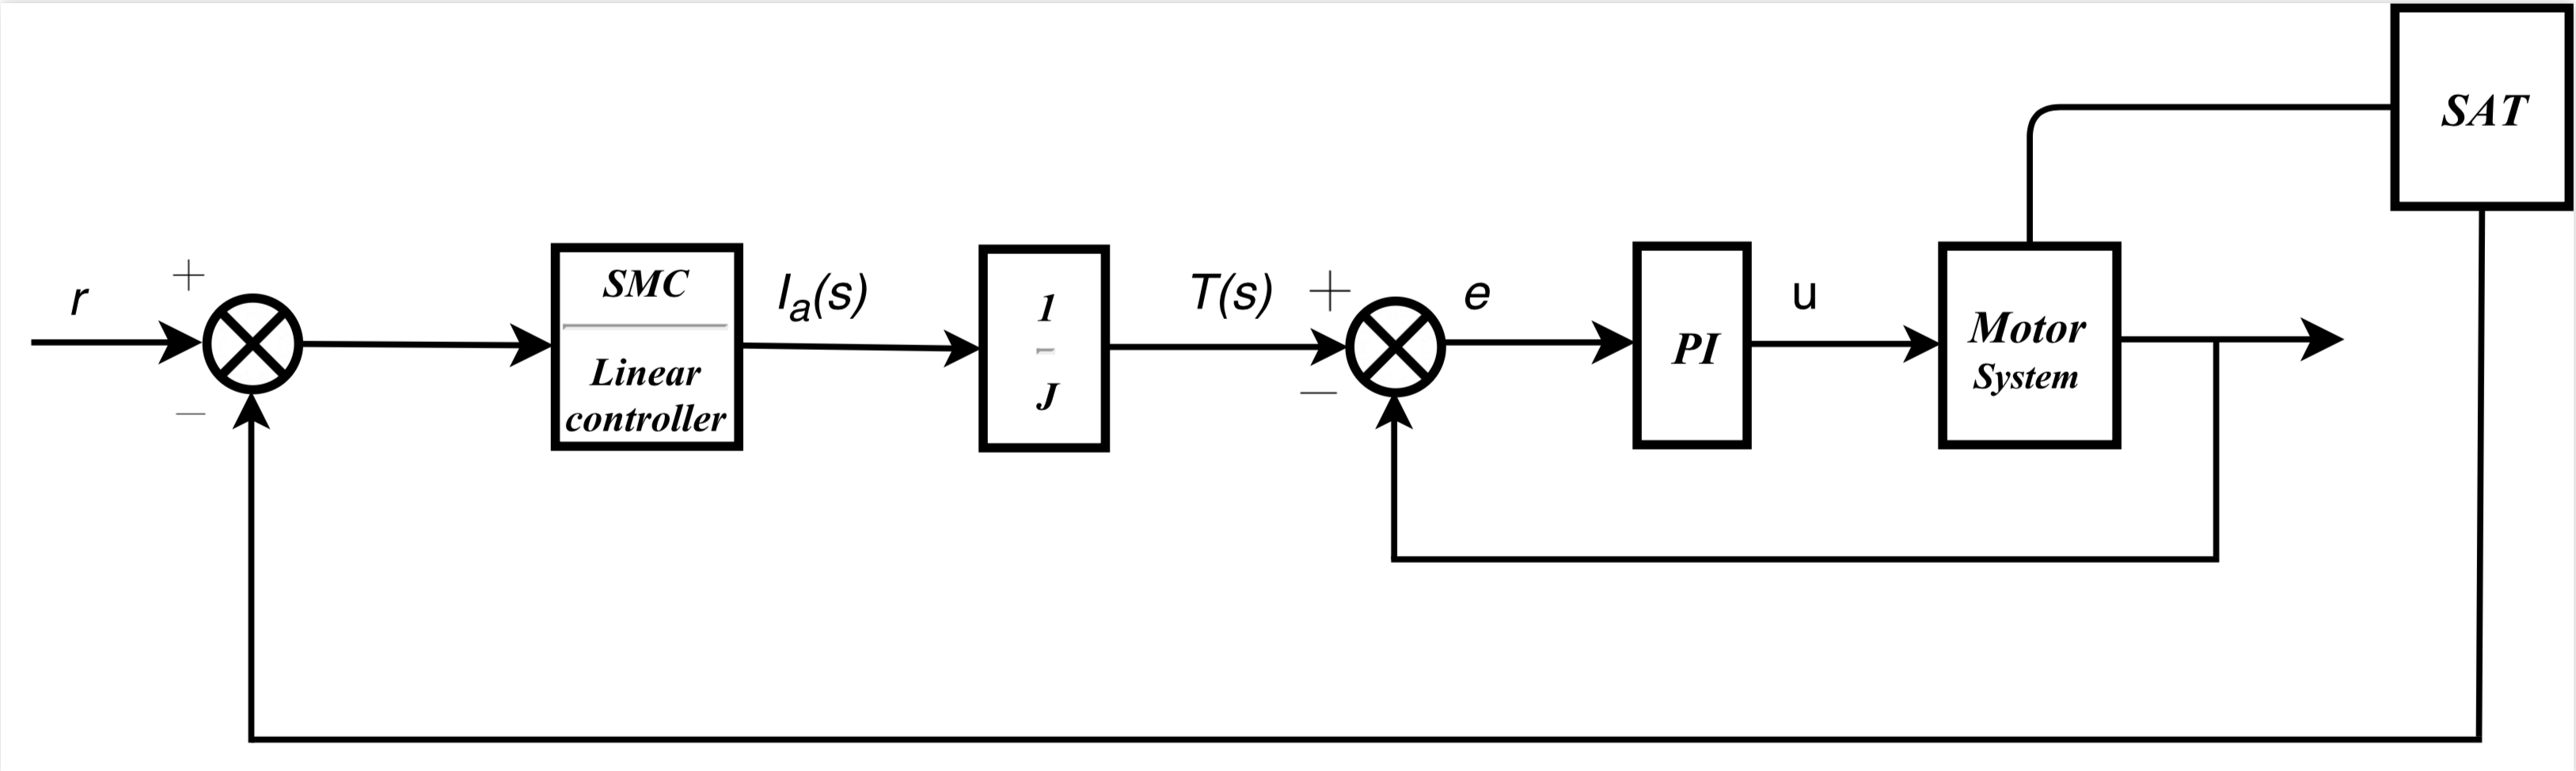
\includegraphics[width=1.0\linewidth]{figures/block_diagram_2}
	\caption{Block diagram of the motor control with PID controller}
	\label{fig:blockdi222}
\end{figure}  
%
The PI controller gains are chosen based on the open loop system response using the Ziegler-Nichols method \cite{PID_tuning} and by trial and error in order to achieve faster closed loop response and asymptotically stable system. The gains are chosen to be:   
%
\begin{flalign*}
	k_{p} = 3.4 \\ k_{i} = 0.9
\end{flalign*}

\todo{make figure bigger}
The root locus of one motor with PI controller is seen in the \figref{fig:rlocus33}
%
\begin{figure}[H]
	\centering
	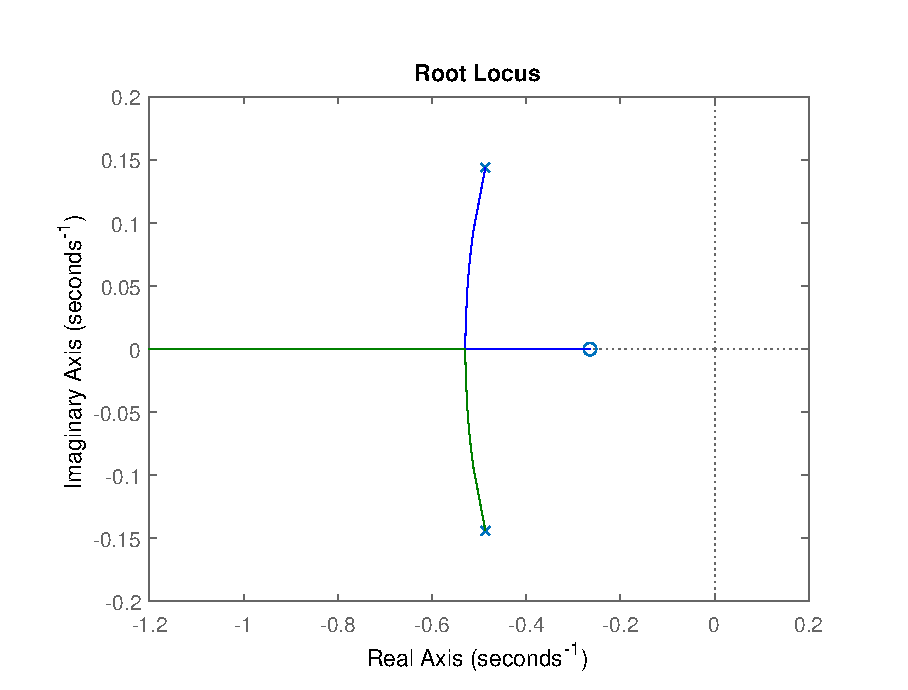
\includegraphics[width=0.7\linewidth]{figures/pid_rootlocus}
	\caption{Root locus of one motor with PI controller}
	\label{fig:rlocus33}
\end{figure}
%
The closed loop system gives complex eigenvalues and fast response and is stable for a wide range of the adjustable parameters. 
%

%
